\documentclass[a4paper, 11pt, twocolumn]{article}
\usepackage[margin=1in, left=15mm, right=15mm]{geometry}       % For setting margins

\usepackage[spanish]{babel}
\usepackage[T1]{fontenc}
\usepackage[utf8]{inputenc}
\usepackage{amsmath, bm}
\usepackage{graphicx}
\graphicspath{{figs/}}
\usepackage{solarized-light} %% codigo fuente
\usepackage[colorinlistoftodos]{todonotes}
\usepackage[colorlinks=true, allcolors=blue]{hyperref}
\usepackage{array}
\usepackage{enumitem} %% listas no numeradas
\usepackage{fancyhdr} %% cabecera personalizada
\usepackage{qtree}
\usepackage{subscript}
\usepackage{tipa}
\usepackage{amssymb}
\usepackage{bbm}

%%%%%%%%%%%%%%%%%%%%%%
% Set up fancy header/footer
\pagestyle{fancy}
\fancyhead[LO,L]{Daniel Quintero}
\fancyhead[CO,C]{Trading Algoritmico - Proyecto Final}
\fancyhead[RO,R]{mayo 2018}
\fancyfoot[LO,L]{}
\fancyfoot[CO,C]{\thepage}
\fancyfoot[RO,R]{}
\renewcommand{\headrulewidth}{0.4pt}
\renewcommand{\footrulewidth}{0.4pt}
%%%%%%%%%%%%%%%%%%%%%%%%%%%%%%%%%%%%%%%%%%%%%%%%%%%%%%%%%%%%%%%%%%%%%%%%%%%%%%%%%%%%%%%%

\title{Trading Algoritmico - Proyecto Final}
\author{Daniel Quintero}
\date{mayo 2018}

\begin{document}
\maketitle

\section{Introducción}
Este documento presenta la implementación de un algoritmo de trading utilizando una estrategia basada en el estado de animo del mercado, realizado en la plataforma Quantopian\footnote{url a quantopian}

\section{Estrategia}
La premisa básica es utilizar información que provea medidas del sentimiento o estado de animo del mercado, detectar cambios de tendencia en estos sentimientos, y a partir de estos cambios crear señales de negociación para establecer posiciones en un activo definido.

Así por ejemplo, si se detecta un incremento en el animo alcista \textit{bullish}, es posible inferir que existen incentivos para que el mercado tome posiciones largas, elevando el precio del activo

Por el contrario, si en el mercado surge un estado de animo a la baja \textit{bearish}, puede que el mercado tome posiciones cortas, liquidando posiciones sobre el activo y llevando el precio de este a la baja

\section{Datos}
Los datos del estado de animo del mercado en Quantopian son proveídos por PsychSignal, quien ofrece tres conjuntos de datos diferentes:

\begin{itemize}
    \item StockTwits Trader Mood: el estado de animo de los \textit{traders} que realizan publicaciones en la plataforma StockTwits
    \item Twitter Trader Mood (All Fields, no Retweets): el estado de animo calculado a partir de \textit{trinos} escritos por traders en twitter.
    \item Twitter Trader Mood (All Fields, with Retweets): similar al anterior, pero incluyendo retweets en los calculos
\end{itemize}

En estos tres conjuntos de datos se tienen las siguientes medidas o variables, las cuales estan calculadas para los principales activos del mercado de acciones estadounidense
\begin{itemize}
    \item bull\_scored\_messages: numero de mensajes identificados con sentimiento bullish
    \item bear\_scored\_messages: numero de mensajes identificados con sentimiento bearish
    \item total\_scanned\_messages: numero total de mensajes analizados
\end{itemize}

Los datos del estado de animo del mercado seleccionados para crear la estrategia son los de \textit{StockTwits Trader Mood}\footnote{https://www.quantopian.com/data/psychsignal/stocktwits}

Con respecto al activo a transar, para este ejercicio, se selecciono el ETF del indice S&P500 (SPY)

\section{Quantopian}
Es una plataforma que crear algoritmos de trading utilizando los conjuntos de datos que tiene disponibles, así como una librería de python propia (zipline) para importar estos datos al algoritmo, calcular indicadores de análisis, y realizar las ordenes.

Quantopian ofrece dos ambientes de desarrollo, con sus propias clases, distinguidos según las necesidades:
\begin{itemize}
    \item El ambiente de investigación (Research Environment): es un notebook de jupyter personalizado, diseñado para hacer exploración y análisis de datos, y establecer posibles estrategias de trading
    \item El entorno de desarrollo (IDE): es donde se programan los algoritmos de trading y se realiza el backtesting del mismo
\end{itemize}

Para este trabajo, si bien se realizaron algunas pruebas en el entorno de investigación importando los datos de sentimiento del mercado y del activo seleccionado, se muestra únicamente el algoritmo creado en el entorno de desarrollo.

\subsection{La clase Pipeline}
Esta clase permite:

\begin{itemize}
    \item Acceder a un conjunto de datos especificado de forma secuencial, para ser procesados por el algoritmo
    \item Calcular métricas establecidas \textit{(factors)}, como por ejemplo retornos, medias móviles e indicadores de análisis
\end{itemize}

\section{Descarga de datos}
Siguiendo la recomendación, se uso pandas\_datareader para descargar los datos del indice Dow Jones, seleccionando el precio de cierre (Adj Close)

\lstset{columns=fullflexible, xleftmargin=1cm, basicstyle=\footnotesize, language=Python, breaklines=true, numbers=left} 
\begin{lstlisting}
# pipeline objects
from quantopian.algorithm import attach_pipeline, pipeline_output
from quantopian.pipeline import Pipeline
from quantopian.pipeline.factors import SimpleMovingAverage, EWMA
#from quantopian.pipeline.data.psychsignal import twitter_noretweets_free as psychsignal # Sentiment data
from quantopian.pipeline.data.psychsignal import stocktwits as psychsignal # Sentiment data
\end{lstlisting}

\section{Datos de trends}
Con el método de read\_csv de pandas se carga a un dataframe el archivo con los datos de las tendencias de Google. Se ajusta el indice del dataframe para usar las fechas de la columna \textit{Mes}

\begin{lstlisting}
def initialize(context):
    context.asset = symbol('SPY')
    sma = SimpleMovingAverage(inputs=[psychsignal.bull_minus_bear], window_length=5)
    ewma = EWMA.from_span(inputs=[psychsignal.bull_minus_bear], window_length=5, span=5)
    
    pipe_columns = {
        'sentiment':psychsignal.bull_minus_bear.latest,
        'msg_volume'  :psychsignal.total_scanned_messages.latest,
        'sma' :sma,
        'ewma' :ewma,
    }
    
    # Attaching our pipeline
    pipe = Pipeline(columns = pipe_columns)
    pipe = attach_pipeline(pipe, name='sentiment')
    schedule_function(rebalance, date_rules.every_day(), time_rules.market_open())
\end{lstlisting}

\begin{lstlisting}
def before_trading_start(context, data):
    # Grabbing the results of our pipeline and removing any NaNs we may find
    context.pipe = pipeline_output('sentiment').dropna().loc[context.asset]
\end{lstlisting}

\begin{lstlisting}
def before_trading_start(context, data):
    # Grabbing the results of our pipeline and removing any NaNs we may find
    context.pipe = pipeline_output('sentiment').dropna().loc[context.asset]
\end{lstlisting}

\begin{lstlisting}
def rebalance(context, data):
    current_position = context.portfolio.positions[context.asset].amount
    buy = False
    sell = False
        
    # rebalance portfolio
    if context.pipe.sentiment > context.pipe.sma and current_position <= 0:
        order_target_percent(context.asset, 1)
        buy = True
        sell = False
    elif context.pipe.sentiment < context.pipe.sma and current_position >= 0:
        order_target(context.asset, 0)
        buy = False
        sell = True
        
    record(sentiment=context.pipe.sentiment, sma=context.pipe.sma, ewma=context.pipe.ewma)
    log.info("Sentiment: " + str(context.pipe.sentiment))
    log.info("sma: " + str(context.pipe.sma) + ", ewm: " + str(context.pipe.ewma))
\end{lstlisting}


\section{Estrategia y señales}
Siguiendo las indicaciones, se calculan los promedios mediante \textit{rolling windows} de tres periodos para los datos de tendencias semanales creados anteriormente, y aplicando \textit{shift} para facilitar la creación de las señales.
Las señales se calculan con la resta de las medias móviles menos el valor de las tendencias, de esta forma se aplica la regla de comparar el valor de la tendencia actual contra el promedio de los tres periodos anteriores

Al vector de señales se aplica la función sign de numpy, que devuelve valores de $-1$ o $1$ si el valor ingresado es menor o mayor a cero respectivamente
\begin{lstlisting}
# first 2 observations are lost plus shift to fit values
trends_ma = trends_week.rolling(window=3).mean().shift(1)
signal = trends_ma - trends_week
signal = signal.apply(np.sign)
\end{lstlisting}

A continuación se muestra el gráfico tanto de las tendencias y las medias móviles calculadas, como de la posición sobre el activo.
\begin{figure}[ht]
\centering
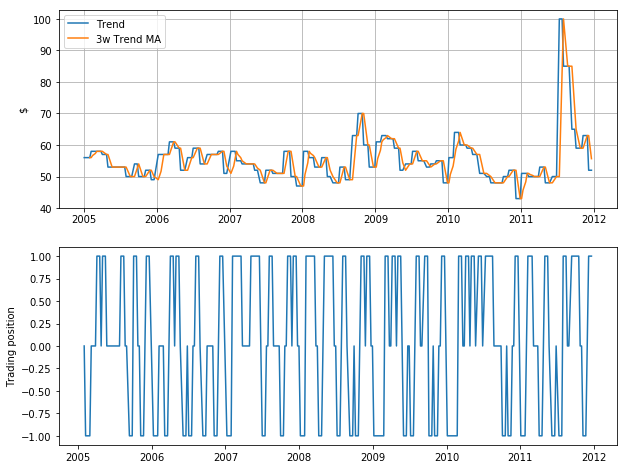
\includegraphics[width=0.5\textwidth]{fig6.png}
\end{figure}

\section{Retornos diarios}


\begin{figure}[ht]
\centering
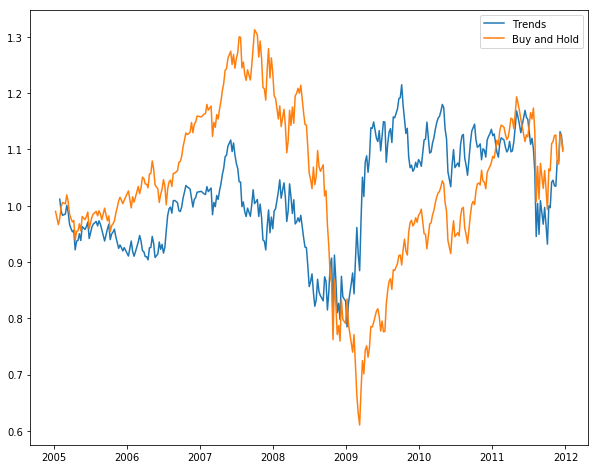
\includegraphics[width=0.5\textwidth]{fig8.png}
\end{figure}

\section{Conclusiones}
Esta estrategia podría entenderse como una versión simplificada de un análisis de sentimiento, en la medida que las tendencias de búsqueda de un termino están relacionadas con un sentimiento positivo o negativo sobre la ocurrencia de algún evento o hecho. De esta forma, dichas tendencias pueden estar relacionadas con los comportamientos de activos financieros. Esta relación puede verse con el ejemplo propuesto de las tendencias de QE y el indice NYSE Composite.

También hay que tener en cuenta otros posibles indicadores a aplicar sobre los datos de tendencias, que puedan mejorar el desempeño de la estrategia de inversión.

Otro posible escenario podría ser utilizar dos tendencias de términos que sean uno opuesto al otro, y realizar una estrategia de tipo \textit{Pairs Trading}.
\end{document}


